% Chapter 1

\chapter{Introduction} % Main chapter title

\label{Chapter1} % For referencing the chapter elsewhere, use \ref{Chapter1} 

\lhead{Chapter 1. \emph{Introduction}} % This is for the header on each page - perhaps a shortened title

%----------------------------------------------------------------------------------------
%\DeclareMathOperator*{\Min}{Min}
The problem addressed is to find a local minimizer of the nonsmooth minimization problem

\begin{equation} \label{mainproblem}
  \begin{aligned}
    & \underset{x \in \mathbb{R}^n}{\text{min}}
    & & f(x) \\
    & \text{s.t.}
    & & l_i \leq x_i \leq u_i , \; \\
    & & & i = 1, \ldots, n.
  \end{aligned}
\end{equation}

where $f \colon \mathbb{R}^n \to \mathbb{R}$, is continuous but not differentiable everywhere and $n$ is a very large but finite number.

The $L-BFGS-B$ algorithm \citep{lbfgsboriginal} is a standard method for solving large instances of \ref{mainproblem} when $f$ is a smooth function. The original name of $BFGS$ stands for Broyden, Fletcher, Goldfarb and Shanno, the authors
of the original "BFGS" quasi-Newton algorithm for unconstrained
optimization discovered and published
independently by them in 1970 [give the 4 references here].
This method requires storing and updating a matrix which 
approximates the inverse of the Hessian matrix $\nabla^2 f(x)$ and
hence requires $\mathcal{O}(n^2)$ operations per iteration.  
The $L-BFGS$ variant [give reference] is based on BFGS
but requires only $\mathcal{O}(mn)$ operations per iteration: thus,
the L stands for Large.  Finally, the last letter B in 
$L-BFGS-B$ stands for bounds, meaning the lower and upper
bounds $l_i$ and $u_i$ in \ref{mainproblem}.  $The L-BFGS-B$ algorithm
is implemented in a well known $FORTRAN$ software package
by the same name [give reference].

In this thesis, there is a brief description of the $L-BFGS-B$ algorithm
at a high level and then explain how the modified algorithm
is more suitable for functions $f$ which may not be
differentiable at their local or global optimizers.  
We call the new algorithm L-BFGS-B-NS where NS stands for
Non-Smooth.  We implemented these changes in a modified version 
of the Fortran code [ref] which is can be downloaded from the website
for this thesis [give URL].  We report on some numerical experiments 
that strongly suggest that the new code should be useful for the
nonsmooth bound-constrained optimization problem (1.1).

We are grateful to Jorge Nocedal and his coauthors for allowing us 
to modify the L-BFGS-B code and post the modified version.  

%\chapter{deleted chapter}

%Larger problems not only mean that their solution will take a longer time to solve. But storing and calculating a the necessary matrices depends on the capabilities of the machine used to solve the problem and this might be prohibitively expensive. There a few large scale optimization techniques that have already been developed for the case when $n$ is very large. Also, several techniques have already been developed to handle this type of problems as long as the function $f$ is smooth. But there is not much out there about large scale problems with nonsmooth $f$

%In this thesis $f(x)$ is a nonsmooth function. This small change will require a few changes in the solution algorithm.

%For the particular case when $n$ is a small number, several methods that solve optimization problems of nondifferentiable functions in lower dimensions \citep{kiwiel85} have been developed. This thesis will try to see if it is possible to bring some of those concepts to large scale optimization. 

%In the case of smooth functions, it is possible to use Newton iteration algorithms and achieve quadratic convergence, the problem with Newton algorithms is that they require second derivatives to be provided\footnote{the main issue with the second derivative is that it requires a total of $n \times n$ partial derivatives. Which is impractical for medium and for some small-size problems}. In the 1950's and several years after that, several "quasi-newton" methods were proposed where the second derivative Hessian matrix is approximated step by step \citep{unconstrained}. These approximations or "updates" are calculated after every iteration of the original algorithm and the way in which this update is found defines a new method depending on the particular needs. This thesis will only be concerned with the $BFGS$. \footnote{BFGS stands for the last names of its authors Broyden, Fletcher, Goldfarb and Shanno} which can achieve super linear convergence, has proven to work in most practical purposes and posseses very nice self correcting features \citep{selfcorrecting}. In $BFGS$, it doesn't matter that one update incorrectly estimates the curvature in the objective function, $BFGS$ will always correct itself in just a few steps. This self-correcting property is very desired in the nonsmooth case, since changes in curvature could be abrupt near the optimal point. 

%$BFGS$ was originally developed for small to medium sized problems, and it is not the right tool for large scale optimization and therefore an $L-BFGS$ adaptation is needed to solve large scale problems\ref{mainproblem}. 

%A final assumption in this thesis is that the Hessian matrix is not sparse. In this case, there are other algorithms that may be more suitable \citep{Fletcher96computingsparse, sparse}, some of them have even been implemented in fortran \citep{lancelot}.

%This thesis builds upon the original $L-BFGS-B$ code \citep{lbfgsbsoftware} that solves smooth problems of $f$. There were three main changes in the code. The first one is the line search descent and curvature conditions which required a weaker version of the curvature in order to satisfy the different structure that a nonsmooth function requires. The second one is the line search methodology which was changed from a cubic interpolation to a bisection algorithm and last change in the thesis was the termination condition.

%Nocedal's original algorithm consists of $2$ steps. In the first step or gradient projection, most of the dimensions in the problem should be removed, making the problem a lot simpler. In the second step there is some fine tuning to guarantee better than just linear speed of convergence.

\chapter{L-BFGS-B}
\label{ChapterConstraints} % For referencing the chapter elsewhere, use \ref{ChapterConstraints} 

This section is a description of the original $L-BFGS-B$ code at a very high level \citep{lbfgsbsoftware}. The original software is intended to work well with smooth functions. This thesis discusses how to modify the algorithm for Non-Smooth functions.

\section{BFGS}

$BFGS$ is a standard tool for optimization of smooth functions.\citep{nocedal} It is a line search method and its goal is to find a search direction starting from its current position $x$. The search direction is of type $d = -B \nabla f$ \footnote{Notice that when $B$ is the identity, this is the same direction as steepest descent. Another common line search method of optimization} where $B$ is an approximation to the inverse Hessian. \footnote{When it is exactly the inverse Hessian the method is known as Newton's method. Newton's method has quadratic convergence but requires the explicit calculation of the Hessian at every single step.} This $k^{th}$ step approximation is calculated via the $BFGS$ formula

\begin{equation} \label{bfgsupdate}
  \begin{aligned}
    B_{k+1} = \left(I - \frac{s_ky_k^T}{y_k^Ts_k} \right) B_k \left( I - \frac{y_ks_k^T}{y_k^Ts_k} \right) + \frac{s_k s_k^T}{y_k^T s_k}
  \end{aligned}
\end{equation}

where $y_k = \nabla f(x_{k+1}) - \nabla f(x_k)$ and $s_k = x_{k+1} - x_k$ and where the first approximation of $B_0$ is assumed to be the the identity matrix $I$ in this thesis.  $BFGS$ exhibits superlinear convergence but it also requires $\mathcal{O}(n^2)$ operations per iteration. \citep{nocedal}

In the case of Non-Smooth functions. $BFGS$ typically succeeds in finding a local minimizer. This however requires some modifications of the line search conditions. This line search conditions is known as the weak Wolfe line search and it will be explained later in this thesis.

\section{L-BFGS}

$L-BFGS$ stands for Limited-memory $BFGS$. This algorithm approximates $BFGS$ using only a limited amout of computer memory to approximate the inverse of the Hessian $B$. So instead of storing a dense $n \times n$ matrix, $L-BFGS$ keeps a record of the last $m$ iterations where $m$ is a small number that is chosen according to the problem at hand. \footnote{In this thesis $m < 20$, and in practice numbers between 5 and 10 are regularly used. There is no way of knowing a priori what choice of $m$ will provide the best results} It is for this reason that during the first $m$ iterations, $BFGS$ and $L-BFGS$ produce exactly the same search directions.

Because of this construction, the $L-BFGS$ algorithm is less computationally intensive and it only requires $\mathcal{O}(mn)$ operations per iteration. So it is much better suited for problems where the number of dimensions $n$ is large. For this reason it is the algorithm of choice in this thesis.

\section{L-BFGS-B}

Finally $L-BFGS-B$ comes naturally as an extension of $L-BFGS$. The $B$ stands for the inclusion of Boundaries.  $L-BFGS-B$ requires two extra steps on top of $L-BFGS$. First, a gradient projection that reduces the dimensionality of the problem. Depending on the problem, the gradient projection could potentially save a lot of iterations by eliminating those variables that are at bound at the optimum. After that, the subspace minimization; here, during the search step phase the step length is restricted as much as necessary in order to remain within the box defined by \ref{mainproblem}.

\subsection{Gradient Projection}
The original algorithm was created for the case when $n$ is large and $f$ is smooth. Its first step is a gradient projection similar to the one outlined in \citep{gradproj1, gradproj2} which is used to determine an active set corresponding to those variables that are on either their lower or upper bounds. The active set defined at point $x^*$ is:

\begin{equation}
  \begin{aligned}
    \mathcal{A}(x^*) = \{ i \in \{1 \ldots n\} |  x^*_i = l_i \vee  x^*_i = u_i\}
  \end{aligned}
\end{equation}

Working with this active set is efficient in large scale problems. A pure line search algorithm would have to choose a step length short enough to remain within the box defined by $u_i$ and $l_i$. So if at the optimum, a large number $\mathcal{B}$ of variables are either on the lower or the upper bound. At least a number $\mathcal{B}$ of iterations might be needed. Gradient projection tries to reduce this number of iterations. In the best case, only $1$ iteration is needed instead of $\mathcal{B}$.

Gradient projection works on the approximation model:

\begin{equation} \label{themodel}
  \begin{aligned}
    m_k(x) = f(x_k) + \nabla f(x_k)^T ( x - x_k) + \frac{(x - x_k)^T H_k (x - x_k) }{2}
  \end{aligned}
\end{equation}

where $H_k$ is a $L-BFGS-B$ approximation to the Hessian $\nabla^2 f$ stored in the implicit way defined by $L-BFGS$.

In this first stage of the algorithm a piecewise linear segment starts on the current point $x_k$ in the direction $-\nabla f(x_k)$. Whenever this direction encounters one of the constraints, the line segment turns corners in order to remain feasible. The path is nothing but the feasible piecewise projection of the negative gradient direction on the constraint box determined by the values $\overrightarrow{l}$ and $\overrightarrow{u}$. At the end of this stage, the value of $x$ that minimizes $m_k(x)$ restricted to this piecewise gradient projection path is known as the 'Cauchy point' $x^c$.

\begin{figure}
\begin{center}
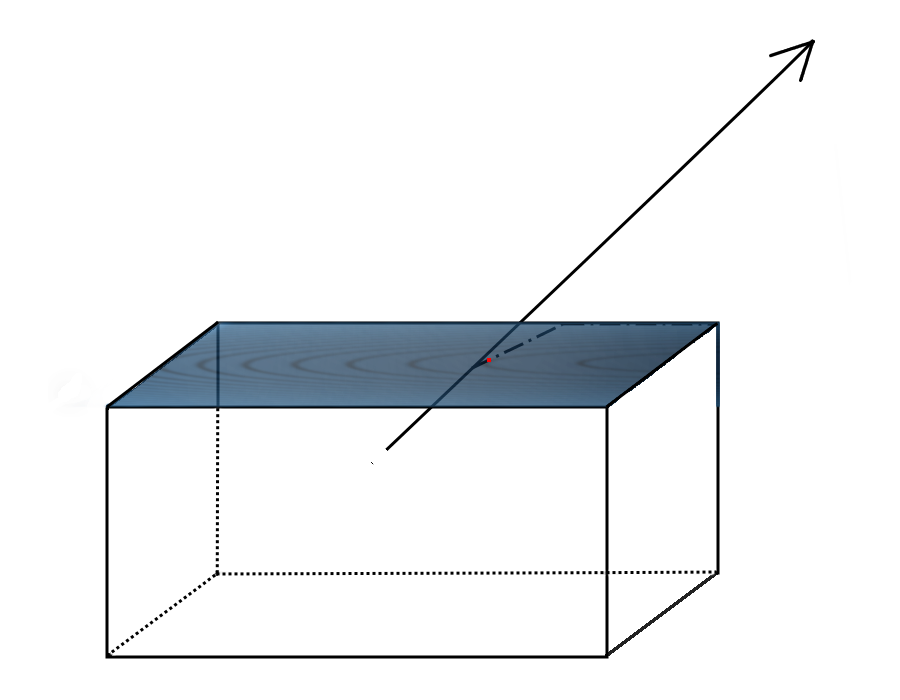
\includegraphics[scale=0.5]{Figures/cajapresentation2.png}
\caption[graph1]{The arrow represents the direction of the gradient. The dotted path represents the projected gradient path from the gradient and onto the box. The region represents the level sets of the model. The optimal point (in red) is the Cauchy point $x^c$}
\end{center}
\end{figure}

\subsection{Subspace Minimization}

The problem with gradient projection is that its search direction does not take advantage of information provided implicitly by $H_k$, and therefore the speed of convergence is at best linear. It is for this reason that a stage two is necessary. Stage 2 or subspace minimization uses an $L-BFGS$ implicit approximation of the Inverse Hessian matrix restricted to the free variables that are not in the active set $\mathcal{A}(x^c)$.

The idea at a higher level is to solve the constrained problem \ref{themodel}, but only on those dimensions that are free. The starting point for this new problem will be the previously found Cauchy point $x^c$, the $L-BFGS$ approximation will provide a new search direction $\hat{d}^u$ that takes implicit advantage of second order approximations of the Hessian matrix.

The algorithm will move in the direction $\hat{d}^* = \alpha^* \hat{d}^u$ where $\alpha^*$ (the step length) is chosen so that the new point $\bar{x}_i$ satisfies weak wolfe descent and curvature conditions, A third restriction on the step length is added so that the next iteration stays feasible. Once this step is finished, the next and final step will be the termination condition. If the termination condition fails a new gradient projection and subspace minimization will be needed.

\chapter{Modifications to the L-BFGS-B algorithm}

We made three main changes to the original $L-BFGS-B$ algorithm. They concern the line search Wolfe conditions, the line search methodology, and the termination condition.

\section{The Wolfe conditions}

Probably the most important change made to the original code was the change in the curvature condition. It is accepted that the Wolfe conditions work very well whenever the function $f$ is smooth \citep{MR1855221}. Originally there are two Wolfe conditions: one of them is the Armijo condition, also known as the sufficient decrease requirement. The other one is the curvature condition, of which the most popular version is the ``strong Wolfe'' curvature condition:

\begin{equation}
  \begin{aligned}
    |d_k^T \nabla f(x_k + \alpha _k d_k)| \leq |d_k^T \nabla f(x_k)|
  \end{aligned}
\end{equation}

Where $d_k$ represents the search direction. The strong Wolfe condition is natural for smooth optimization. Its goal is to find a step length long enough that the slope has been reduced ``sufficiently'', but the problem is that it does not work well for the Non-Smooth case. This is because near the minimal points, there may be abrupt changes in the gradient. For example the curvature condition can never be satisfied when $f(x) = |x|$, because the slope never becomes flat. The ``weak wolfe'' condition

\begin{equation}
  \begin{aligned}
    d_k^T \nabla f(x_k + \alpha _k d_k) \geq d_k^T \nabla f(x_k)
  \end{aligned}
\end{equation}

is all that is needed to guarantee that the $BFGS$ updated inverse Hessian approximation is positive definite \citep{overtonlewis}. This weak version is the one that will be used in this thesis. It was changed inside of the line search algorithm explained in the next section.

\section{The line search methodology}

The original $FORTRAN$ code \citep{lbfgsbsoftware} contains a line search subroutine. This subroutine first establishes a maximum step. This maximum step is such that it guarantees that the step length stays within the bounding box delimited by $l$ and $u$. This part of the line search was not changed in this thesis. The next part of the line search is finding a step length that satisfies a decrease and a curvature condition (aka. Armijo and Wolfe conditions). The next procedure was completely changed for the purpose of this thesis. and is only explained here with the purpose of showing why it needed to be modified. It was called on line $2662$ \ref{ignoredcode} of $lbfgsnomessages.f90$ and it has been left commented out in order to show how this call was before the modifications.

From then on, the line search required a lot of modifications. This new code is available online \citep{lbfgsbNS}

The original line search was a two stage process. In the first stage the interval was chosen so that it contains a minimizer of the modified function, which is nothing but a modification of the Armijo condition.

\begin{equation} \label{armijomod}
  \begin{aligned}
    \Psi(\alpha_k) = f(x_k + \alpha_k d_k) - f(x_k) - c1 \alpha_k d_k^T  \nabla f(x_k)
  \end{aligned}
\end{equation} 

If $\Psi(\alpha_k) < 0$ and $\alpha_k d_k^T \nabla f(x_k) > 0$. The interval is chosen so that it contains a minimizer of f. This first stage took place in the subroutine $dcsrch$; specifically on lines $3687$ and $3709$ \ref{stage1}

The second stage was called on line $3713$ and its mission was to find the step that satisfied Armijo and ``Strong'' Wolfe conditions on the original function (as opposed to the modified from stage 1) $f$. Both stage 1 and stage 2 called the subroutine $dcstep$. The subroutine still exists on file $lbfgsbnomessages.f90$ for illustration. Although it is never called in this thesis.

But there is a problem with the function $dcstep$. It turns out that function $dcstep$ was designed to work only with smooth functions in mind. The code takes advantage of quadratic and cubic approximations to the function in order to calculate the next points that satisfy armijo and wolfe conditions. Unfortunately, these second and third order approximations do not work in the Non-Smooth case, and the optimizer crashes under the line search as it was formulated. Function $dcstep$ starts on line $3779$ and a sample of the approximations is shown in between lines $3881$ and $3902$ \ref{nsnowork} of $lbfgsbnomessages.f90$.

The approach to this issue is to use a line search similar to the one in hanso \citep{hanso}. The HANSO approach is to double the step length while the Armijo condition is violated (while the decresing conditions has not been satisfied). And once the interval has been bracketed, to do a bisection until both Armijo and Wolfe conditions are satisfied. The only difference with the HANSO approach in this thesis is that the line search in HANSO can double its step length up to $30$ times \footnote{for all practical purposes this is considered as a good limit of iterations}. Whereas in this thesis, the step length can double only as long as the step length is less than the maximum value that guarantees feasibility of the solution. This version of the bisection and expansion is found in between lines $4425$ and $4456$ \ref{linesww} of $lbfgsbnomessages.f90$


\section{The termination condition}

One important requirement of a practical algorithm is that it ends in a finite time. For the case of smooth functions, the usual way to check whether the algorithm has converged, is by using the projected gradient which is nothing but the projection of the negative gradient onto the bounding box defined by $l$ and $u$. If this projected gradient has a small norm the algorithm has converged. In the case of nonsmooth functions however, this is not necessarily true and the function at the minimum, may have a wedge. In this wedge the projected gradient may not vanish. Furthermore, if there is a sequence of points that approaches the optimum $x$ from the right, the projected gradients corresponding to this sequence of points might be completely different from the projected gradients associated to a sequence of points that approach the optimum $x$ from the left.

Given this set of conditions, there is the need for a special set of rules to establish the finalization of each optimization.

\subsection{Description of the Solution}

Overton and Lewis formulate an algorithm that gives a practical solution to this problem on section $6.3$ \citep{overtonlewis}
The best practical methodology should be to calculate wheter zero $0$ or a very small number is the norm of a vector that is part of the convex hull of gradients evaluated at points near the optimum candidate $x$. In order to make sure that the gradient zero $\vec{0}$ or a vector with a very small norm smaller than a very tiny tolerance $\tau_d > 0$ is part of the convex hull calculated near a neighbourhood of the optimum. The algorithm needs to keep a record of the latest gradient vectors in this small neighbourhood of the point where it is suspected that the optimum is located. The neighborhood is defined as those points with a distance to $x$ smaller than a small tolerance $\tau_x > 0$ and no more than $J \in \mathbb{N}$ iterations back.  This list of gradients is referred to as the set $\mathcal{G}$ \citep{overtonlewis}

With this list $\mathcal{G}$ of gradients at hand. The next step is to solve a quadratic program that locates the vector with the minimal norm that lives in the convex hull of these gradients.  If the norm of this vector has a norm smaller than $\tau_d$ , the algorithm ends with a message of convergence success. If the minimum such norm is larger than the tolerance, the algorithm must continue to the following iteration and not terminate.

Every vector in the convex hull can be expressed as a nonnegative linear combination $Gz$ of those vectors in $\mathcal{G}$. Where $G$ is the matrix with columns made up of gradients in $\mathcal{G}$; and $z$ is such that $\sum_{i=1}^n z_i = 1$ and $z_i \geq 0$.

In other words the objective is to find the right combination of $z$ that minimizes the norm $||Gz||_2$.  This is equivalent to solving the optimization problem

\begin{equation} \label{quadraticproblem}
  \begin{aligned}
    & {\text{min}}
    & & q(z) = ||G z ||_2^2 = z^TG^TGz  \\
    & \text{s.t.}
    & & \sum_{i = 1} ^J z_i = 1 \; \\
    & & & z_i >= 0.
  \end{aligned}
\end{equation}

The solution to this problem $z^*$ has the associated vector $Gz^*$. And if $||Gz^*|| < \tau_d$ the algorithm converges.

\subsection{The Solution of the Quadratic Program}

The solution of \ref{quadraticproblem} was implemented with a practical primal-dual methodology. This methodology is the same methodology implemented by Skajaa \citep{skaaja} in his thesis. His code qpspecial was implemented in $FORTRAN$ and is part of $lbfgsbnomessages.f90$. The solution is a typical Mehrotra's Predictor-Corrector algorithm applied to quadratic programming.

This algorithm initially tries to solve the Karush Kuhn Tucker $KKT$ conditions. The $KKT$ is a system of equations whose solution characterizes the solution of the original optimization problem. In \ref{quadraticproblem}. The Karush Kuhn Tucker equations are:

\begin{equation} \label{kkt}
  \begin{aligned}
    G^TGz - e^Ts
    & = & 0 & \\
    \sum_{i = 1}^J x - 1
    & = & 0 & \\
    z_is_i & = & 0 &; &i = 1,2, \dots, J\\
    (s, z) & \geq & 0 &
  \end{aligned}
\end{equation}

Where $s$ is the variable of the dual problem.

In order to solve this system of equations a variant of Newton's method is used. This Newton's method as usual, provides a search direction which requires a corresponding step length.  Since this is an interior point method, it approaches the solution following a path inside the convex interior of the feasible set.  In the best of cases, it would be nice to approach the solution through a \emph{central path} where the third equation in \ref{kkt} is allowed to take more relaxed values $z_is_i = \tau$, where $\tau \geq 0$. If the solution is approached through this \emph{central path}. The convergence will require fewer iterations.

The problem is that the pure Newton's method solution is not close to this central path. The step length is usually very small because of the nature of the third and fourth equations. If the step length is too large, the condition of $z > 0$ or $s > 0$ will be violated. The method by itself approaches the solution very close to the boundaries of the feasible set. Not close to the \emph{central path} where the step lengths could be larger and the convergence therefore would be faster.  It is for this reason that a centering of the path is performed. This first step is known as the ``predictor'' step.

Besides the centering; Mehrotra proposed a ``correction'' stage which pushes the solution closer to the central path by taking into account the curvature of the approaching \emph{central path}. This second stage is also used to calibrate some of the parameters used during the centering in the ``predictor'' stage. The second stage is similar to the first stage in that it requires the solution of a new system of equations.

\begin{figure}
\begin{center}
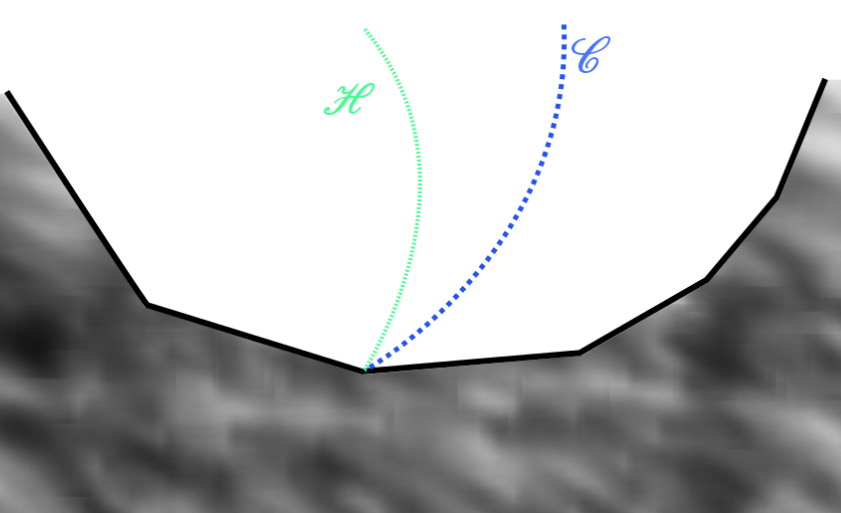
\includegraphics[scale=0.3]{Figures/CentralPath.png}
\caption{The central path $\mathcal{C}$ is approached from a current and noncentral point on the tangent path $\mathcal{H}$}
\end{center}
\end{figure}

The beauty of Mehrotra's algorithm, is that the Cholesky factorization required for the first stage is reused during the second stage, which improves performance.  This algorithm is widely used in optimizers.

\chapter{the solution test functions}

In order to make some tests, a few functions will be evaluated. The most important function to test this non-smooth optimizer is a modified version of rosenbrock's:

\begin{equation}
    f(x) = (x_1 - 1)^2 + \sum_{i = 2}^n |x_i - x_{i - 1}^2|^p
\end{equation}

Where the value of $p$ changes the behaviour of the optimizer. This function can be proven to be lipschitz continuous whenever $p > 1$ if restricted to the domain defined by  

\begin{equation}
  \begin{aligned}
    x_i = 
    \begin{cases}
      [-100, 100] & \text{if } i \in \text{ even numbers} \\
      [10, 100] & \text{if } i \in \text{ odd numbers}
    \end{cases}
  \end{aligned}
\end{equation}

and in fact, whenever the function is restricted to a finite domain this function will be lipschitz continuous for $p > 1$. Whenever $p > 1$ the function $f(z) = |z|^p$ is zero $0$ around zero because the derivative $p |z| ^{p-1}$ is zero whenever $z$ tends to zero from the right. (this is also the case from the left because it is an even function). However the second derivative will not be as nice.

For the case when $p \leq 1$ the second derivative tends to infinity. $\displaystyle \lim_{x \to 0^+} {f' = \infty}$. Which is already well known given the "heavyside" look of $f(z) = |z|$.

The convergence of the algorithm smoothly descends to the objective 

\begin{center}
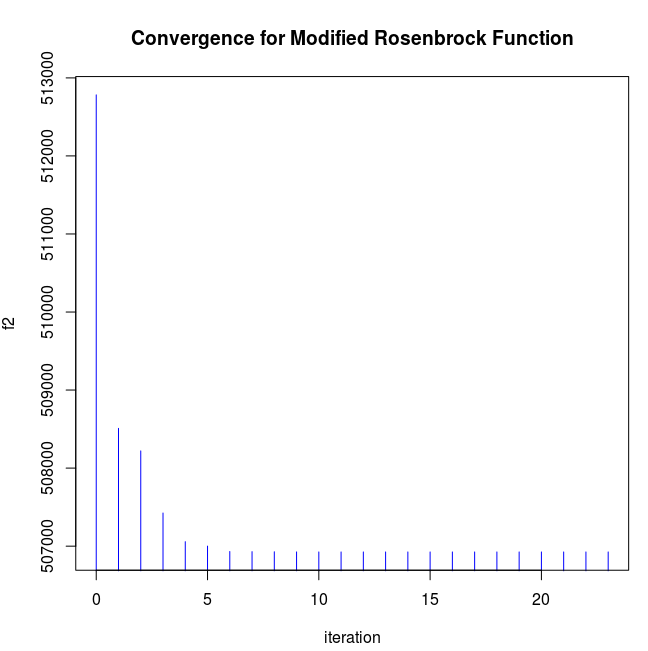
\includegraphics[scale=0.3]{Figures/convergence.png}
\end{center}

The converge is adversely affected by the selection of $p$ as one would expect. Values of $p$ descending to $1$ make the function less "smooth" and have the adverse effect of making the convergence much more difficult. In this exercise it is noticeable how slow the convergence becomes for a few specific values of $p$. In particular for $1.0001$

\begin{center}
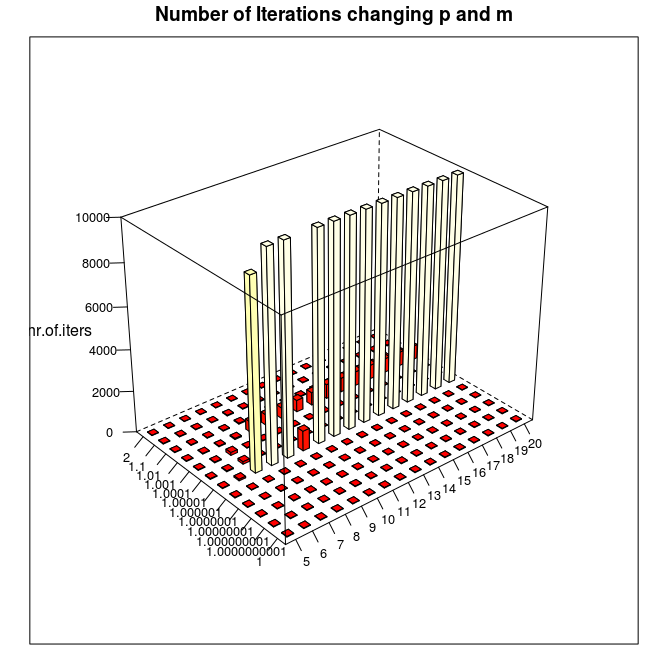
\includegraphics[scale=0.3]{Figures/hist3dmpniter.png}
\end{center}

\begin{equation}
  \begin{aligned}
    f(x_k + \alpha_kp_k) \leq f(x_k) + c_1 \alpha _k p_k^T\nabla f(x_k)
  \end{aligned}
\end{equation}

